\documentclass[11pt]{article}
\usepackage{amsmath,amssymb,amsthm}
\usepackage[margin=1.05in]{geometry}
\usepackage{graphicx}
\usepackage{booktabs}
\usepackage{microtype}
\usepackage[colorlinks=true,linkcolor=blue,citecolor=blue,urlcolor=blue]{hyperref}

\newtheorem{theorem}{Theorem}
\newtheorem{lemma}{Lemma}
\newtheorem{definition}{Definition}
\newcommand{\R}{\mathbb{R}}
\newcommand{\thit}{t_{\mathrm{hit}}}
\newcommand{\texit}{t_{\mathrm{exit}}}
\newcommand{\trel}{t_{\mathrm{release}}}

\title{An entry--exit law for dead-neuron resurrection:\\
the smoothed-ReLU limit of training dynamics at an activation\\
boundary, and its confirmation in a small MLP and a\\
one-layer transformer}
\author{L.~Caloi Santos}
\date{2026-07-25 \quad DRAFT v1 --- not for circulation}

\begin{document}
\maketitle

\begin{abstract}
A neuron ``dies'' when its pre-activation margin crosses zero on all data; for a
hard ReLU the dead unit has exactly zero gradient and never returns. We ask what
governs death and resurrection in the smoothed activations used in practice. For
shallow softplus networks under gradient flow we prove that, in the sharp limit
$\beta\to\infty$ of the activation stiffness, death and resurrection are governed
by a hybrid system \emph{with memory}: the dead unit's parameters freeze and
reactivation occurs exactly when the signed time integral of the excluded
residual returns to zero --- the classical entry--exit function --- with a
universal first-order release coefficient; all constants are verified on one
two-neuron instance. The two limit orders do not commute: the field-first (pointwise generalized-gradient) limit
freezes dead units forever, the smoothed flow revives them by the area law. We
then track the law upward through a pre-registered experimental ladder: a reduced
deterministic-schedule model is falsified under noise; two instrument designs are recorded as
negatives (a calibrated null fires); and a confirmatory MLP run ($400$ runs,
$T=0$) reproduces resurrection at $p=0.50$ with the residual area opening before
$13/16$ returns, hard ReLU giving zero, and a monotone channel staircase in
$\beta$. A pre-registered one-layer-transformer confirmatory ($800$ runs, $T=0$)
then closes the ladder: the theorem's class transfers to the FFN's own channel
(softplus-$\beta3$ with attention frozen, $p_{\mathrm{sust}}=0.440\,[0.300,0.587]$,
drive area opening before the return in $21/22$); an upstream
channel} adds $\approx+0.20$ in all four activation arms --- including hard ReLU,
whose own channel is exactly zero; and the GELU sign-flip barrier is
\emph{consistent with}, not established by, the counts, which are confounded with
injection depth, while its sign signature separates deep from shallow in $92\%$
against $4\%$.
\end{abstract}

\section{Introduction}\label{sec:intro}

Write $\Phi:\mathcal{W}\to\mathcal{F}$ for the parametrization of a network and
$J=D\Phi$ for its Jacobian. A neuron whose pre-activation margin is negative on
every datum contributes an identically zero column to $J$: it sits on a stratum
of the singular locus where $J$ drops rank. Under a hard ReLU the gradient of the
loss in the directions of that unit is exactly zero, so the stratum is
\emph{absorbing} --- a dead unit stays dead. This is the mechanism behind the
empirically documented dormant-neuron and loss-of-plasticity
phenomena~\cite{Sokar23,Lyle23,Dohare24}. The question of this paper is what
replaces the absorbing stratum when the activation is \emph{smoothed}, as it is
in every softplus/GELU network actually trained.

Our answer is an exact gating law and its numerical arc. The contributions are:

\begin{itemize}
\item \textbf{A theorem (\S\ref{sec:theorem}, Thm.~\ref{thm:main}).} In the sharp
limit $\beta\to\infty$ of a shallow softplus network under gradient flow, the
death/resurrection of a neuron is the entry--exit problem of a slow--fast system:
the dead unit freezes and reactivates when $\int R\,dt=0$, where $R$ is the
residual excluding that unit. The uniform rate is $O(\log\beta/\beta)$, the
release time carries a \emph{universal} first-order coefficient
$-1/(cR(\texit))$, and the law is independent of the smoothing within the
monotone-sigmoid class (softplus, erf); GELU is excluded because its derivative
is non-monotone. Six lemmas, each with an executable verification (the exit-corner half of the corner lemma is verified indirectly, through the release times), are
summarized in \S\ref{sec:theorem} and stated in Appendix~\ref{app:lemmas};
Figs.~\ref{fig:mecanismo}--\ref{fig:constantes} show the mechanism and the
predicted constants.

\item \textbf{Non-commutation (\S\ref{sec:noncomm}).} The two limit orders
(smooth-then-sharp vs.\ the pointwise generalized-gradient flow) do not commute.
The field-first order is the frozen branch of Eberle, Jentzen, Riekert and
Weiss~\cite{EJRW23}; our flow-first limit resurrects. This is the exact
mathematical content of ``dead ReLU units stay dead, smooth units come back.''

\item \textbf{A pre-registered experimental ladder (\S\ref{sec:experiments}).}
Organized by prediction, with the null controls and the negatives shown:
a reduced deterministic-schedule model \emph{falsified} under SGLD
(\S\ref{sec:falsif}); two instrument designs recorded as \emph{negatives} because
a calibrated null fired (\S\ref{sec:negativos}); the mechanism first observed in
an MLP pressure pilot (\S\ref{sec:mecanismo}); and a \emph{confirmatory} MLP run
--- $400$ runs, area law reproduced with confidence intervals, hard ReLU as the
zero-gradient control, monotone staircase in $\beta$ (\S\ref{sec:confirm},
Fig.~\ref{fig:escada}); and a \emph{confirmatory} one-layer transformer ---
$800$ runs, the theorem's class transferring in the FFN's own channel, a
upstream channel adding the same $\approx+0.20$ in all four arms, and the GELU barrier reported as
consistent-with-barrier under an explicit depth confound
(\S\ref{sec:transformer}), whose scoping had already exposed both new mechanisms.
\end{itemize}

The paper is deliberately honest about scope: the theorem is one two-neuron
instance; the confirmatories are two small architectures at temperature zero; the
stochastic gate is open and, where we probed it, it \emph{breaks} the
deterministic schedule (\S\ref{sec:falsif}).

\section{Setup and notation}\label{sec:setup}

Data $(x_i,y_i)_{i=1}^n$ in general position; shallow network
$f_\theta(x)=\sum_k g_\beta(w_kx+b_k)$ with softplus
$g_\beta(z)=\beta^{-1}\log(1+e^{\beta z})$ (general monotone sigmoids in
\S\ref{sec:theorem}); quadratic loss
$L=\tfrac1{2n}\sum_i(f_\theta(x_i)-y_i)^2$; gradient flow $\dot\theta=-\nabla L$.
The parameter $\beta$ is the \emph{activation stiffness}: as $\beta\to\infty$,
$g_\beta\to\mathrm{ReLU}$ and $g_\beta'\to\mathbf 1_{\{z>0\}}$.

Fix one neuron $A$ and one datum $j$. Its \emph{margin} is
$z=\theta_A\cdot(x_j,1)$; write $c=\|(x_j,1)\|^2/n$ and let
\[
R(t)=y_j-f_{-A}\bigl(x_j;\theta_B(t)\bigr)
\]
be the \emph{residual excluding $A$} ($\theta_B$ collects the other parameters).
The \emph{hybrid reference} $\theta^{\mathrm{hyb}}$ runs the full ReLU flow until
the first time $\thit$ with $z=0$, then freezes $\theta_A$ and runs $\theta_B$
alone; set $R^{\mathrm{hyb}}$ accordingly and
$A^{\mathrm{hyb}}(t)=\int_{\thit}^t R^{\mathrm{hyb}}$ for its signed area. The
death of $A$ is exactly the rank drop of $J$ on the stratum $\{z\le0\}$; the
question is the fate of the trajectory on that stratum.

\paragraph{Hypotheses.}
\textbf{(H1)} $R^{\mathrm{hyb}}(\thit)<0$ (transversal death).
\textbf{(H2)} $A^{\mathrm{hyb}}$ has a first zero at $\texit<T$ with
$R^{\mathrm{hyb}}(\texit)>0$ and $A^{\mathrm{hyb}}<0$ on $(\thit,\texit)$.
\textbf{(H3)} the other margins of $A$ stay $\le-\delta_1<0$ on the episode.
\textbf{(H4)} no other switching event occurs in $[0,T]$.

\section{The entry--exit theorem}\label{sec:theorem}

\begin{definition}[hybrid limit]\label{def:hybrid}
$\theta^\infty$ equals: the ReLU flow on $[0,\thit]$; on $[\thit,\texit]$,
$\theta_A\equiv\theta_A(\thit)$ (frozen) with $\theta_B$ the $B$-only flow; on
$[\texit,T]$, the ReLU flow restarted at
$(\theta_A(\thit),\theta_B^{\mathrm{hyb}}(\texit))$.
\end{definition}

\begin{theorem}[$T2'$-min]\label{thm:main}
Under (H1)--(H4), for every $\delta>0$,
\[
\sup_{t\in[0,T]\setminus(B_\delta(\thit)\cup B_\delta(\texit))}
\|\theta^\beta(t)-\theta^\infty(t)\| = O_\delta\!\left(\tfrac{\log\beta}{\beta}\right),
\qquad
t^\beta_{\mathrm{release}}=\texit-\frac{1}{c\,R^{\mathrm{hyb}}(\texit)}\cdot\frac{1}{\beta}
+o(\beta^{-1}),
\]
where $t^\beta_{\mathrm{release}}$ is the first return of the margin $z$ to $0$
after death. The $\log\beta$ in the sup is sharp and is carried solely by the
normal coordinate of $\theta_A$ inside the episode (the sticking depth
$z\sim-\beta^{-1}\log\beta$); $\theta_B$ obeys $O(\log\beta/\beta^{2})$ and the
tangential components of $\theta_A$ are exponentially frozen. The first-order
release coefficient is \emph{universal}: in the product (entry delay $\times$
area cut) the arrival speed cancels, leaving the reciprocal exit speed --- each
corner contributes the reciprocal of its transversal speed. The remainder is
$o(\beta^{-1})$ as proved. The limit is that of the regularized flow taken
first; the field-first (pointwise generalized-gradient) flow freezes the dead
neuron forever --- the two limit orders do not commute (\S\ref{sec:noncomm}).
Discrete hard-ReLU gradient descent freezes it as well, a separate observation
confirmed empirically in \S\ref{sec:confirm}.
\end{theorem}

\begin{figure}[t]
\centering
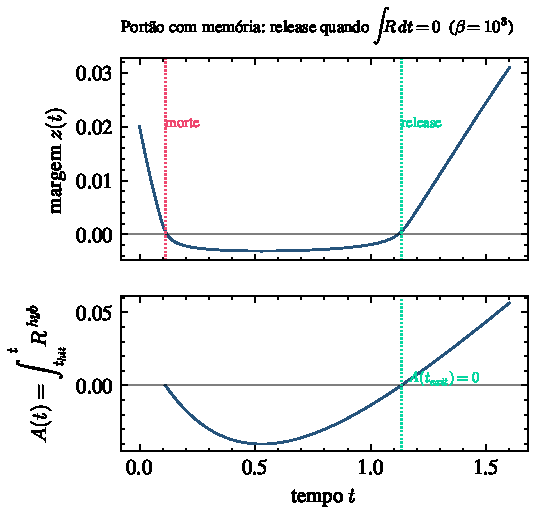
\includegraphics[width=0.60\linewidth]{../t2-prova/fig1-mecanismo.pdf}
\caption{The memory gate at $\beta=10^3$ (coupled system, reference instance).
Top: the margin $z(t)$ dies at $\thit$, hugs the sticking layer of depth
$\sim\beta^{-1}\log\beta$, and releases. Bottom: the hybrid area
$A(t)=\int_{\thit}^t R^{\mathrm{hyb}}$; release coincides with $A=0$ up to
$O(\beta^{-1})$ (Thm.~\ref{thm:main}). Deterministic Euler integration
($dt=10^{-5}$); uncertainty is discretization only. Script
\texttt{t2-prova/figuras\_draft.py} (committed).}
\label{fig:mecanismo}
\end{figure}

\paragraph{Proof outline.}
The episode reduces to a scalar entry--exit problem through six lemmas
(Appendix~\ref{app:lemmas}); each has a committed executable
symbolic/numeric verification (\texttt{passo0--6}, \texttt{prova\_L1--L6}). In
the gauge $w=e^{\beta z}$, fast time $\tau=\beta t$, the margin obeys the
quadratic normal form of De Maesschalck--Schecter~\cite{DMS16} with
$\varepsilon=\beta^{-1}$ (Lem.~\ref{lem:gauge}); with $u=1/w$ and
$\Phi(u)=\log u+u$ one has the exact additive quadrature
$d\Phi/dt=-c\beta R+c\log(1+w)$, so the layer is held by the \emph{area}, not by
the sign of $R$ (Lem.~\ref{lem:release}): $u(t)=c\beta|A(t)|(1+o(1))$ returns to
$O(1)$ at $\texit+O(\beta^{-1})$. The $B$-subsystem is affine and, conditionally
on the layer being maintained, tracks the hybrid at $O(\log\beta/\beta^2)$
(Lem.~\ref{lem:gronwall}). A coupled continuation (nonempty--open--closed)
closes the feedback loop and yields the two-term release law
(Lem.~\ref{lem:bootstrap}); the entry and exit corners contribute mirrored
$1/\beta$ terms whose arrival-speed factor cancels
(Lems.~\ref{lem:corner-in},~\ref{lem:corner-out}). The dead face carries an
identically zero field on one side --- a degeneracy outside generic
piecewise-smooth exit theory~\cite{Jef16,GH} and of the exponentially flat type
of Kristiansen~\cite{Kri17}; the canonical Sotomayor--Teixeira
regularization~\cite{ST98,LST07} requires both one-sided normal components
nonzero and so does not cover it. The coupling of the forcing to the flow (the
residual is generated by the very trajectory it gates) has, to our knowledge, no
analogue in the entry--exit literature~\cite{SDR23}.

\begin{figure}[t]
\centering
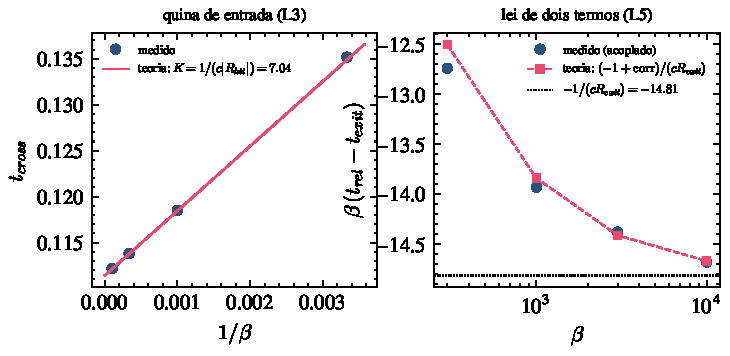
\includegraphics[width=0.95\linewidth]{../t2-prova/fig2-constantes.pdf}
\caption{Predicted constants vs.\ measurements (deterministic runs; uncertainty
is discretization). Left: entry-corner crossing times against $1/\beta$; the
line is the \emph{proved} slope $K=1/(c|R^{\mathrm{hyb}}(\thit)|)=7.04$
(Lem.~\ref{lem:corner-in}), not a fit. Right: the two-term release law
(Lem.~\ref{lem:bootstrap}, squares) against the coupled measurements (circles)
over $\beta\in[3\cdot10^2,10^4]$; dotted line: the universal first-order
coefficient $-1/(cR^{\mathrm{hyb}}(\texit))=-14.81$. Script
\texttt{t2-prova/figuras\_draft.py}.}
\label{fig:constantes}
\end{figure}

\paragraph{Numerical verification (one instance).}
$X=(0.5,1.5)$, $Y=(0.5,1.0)$, $\theta_A(0)=(-0.5,0.27)$,
$\theta_B(0)=(1.144,0.261)$; $\thit=0.1114$, $\texit=1.1325$, $\delta_1=0.508$.
Every empirically measured constant is predicted by the proofs: entry
coefficient $K_{\mathrm{teo}}=7.04$ vs $7.13$ fitted ($1.2\%$); the coupled
two-term law $(-1+\mathrm{corr})/(cR_{\mathrm{exit}})$ reproduces the fine-grid
coupled sweep $-12.74/-13.93/-14.38/-14.68$ at $1.9\%/0.7\%/0.2\%/0.1\%$ for
$\beta=3\cdot10^2\ldots10^4$ (universal coefficient
$1/(cR_{\mathrm{exit}})=14.815$; against $-14.68$ the leading coefficient alone
is at $0.9\%$); tangential drift at machine zero. All numerics are this single
two-neuron instance; breadth is future work.

\paragraph{Regularization independence.}
The release criterion depends only on $\int R\,dt=0$, not on the sigmoid: for the
erf class ($g_\beta'=\Phi_{\mathrm{gauss}}(\beta z)$) the coupled system releases
at the same $\texit$ with $O(\beta^{-1})$ gap (verified). GELU itself,
$z\,\Phi_{\mathrm{gauss}}(z)$, has a non-monotone derivative and is \emph{not} a
member of the family for any $\beta$; \S\ref{sec:transformer} shows this is not a
technicality but a distinct mechanism.

\section{Non-commutation and the plasticity bridge}\label{sec:noncomm}

The theorem is the flow-first limit: take $\beta\to\infty$ of trajectories. The
\emph{field-first} order --- flow the pointwise-limit generalized gradient ---
instead freezes degenerate neurons forever; this is the rigorous branch of
Eberle, Jentzen, Riekert and Weiss~\cite{EJRW23}, whose selected solution has a
non-decreasing degenerate set (the convention $\mathrm{ReLU}'(0)=0$ and the
no-revival mechanism are the same, though their degenerate stratum is the
fully-zero one, not literally our functionally dead neuron). The two orders do
not commute: field-first freezes, flow-first resurrects by the area law.

In machine-learning terms this non-commutation is the statement behind an
empirical trend: discrete ReLU units that die stay dead --- the dormant-neuron
and loss-of-plasticity phenomena documented across deep and reinforcement
learning~\cite{Sokar23,Lyle23,Dohare24}, mitigated in practice by recycling dead
units; the field's concurrent migration to smooth activations is consistent with the mechanism described here --- whereas the smoothed flow
resurrects them by the area law. The channel that reopens a smoothed unit is
$e^{\beta z}$, which closes as $\beta\to\infty$; \S\ref{sec:confirm} measures the
resulting staircase directly, and the most alive arm ($\beta=3$) is the
effective stiffness of the GELU family (GELU $\approx z\,\sigma(1.702z)$, i.e.\ $O(1)$).

\section{Experiments}\label{sec:experiments}

The claims are tested by prediction, each with its null control, and the failed
designs are shown rather than hidden. Every confirmatory analysis was frozen by
a pre-registration commit before the run; hypotheses that fell were archived, not
rewritten. Commits: piloto-pressure \texttt{b48b527}; rate pilot \texttt{995a87c};
4a.3 pre-registration \texttt{a8f8f8c}; 4a.3 confirmatory \texttt{5a961cb};
transformer (etapa-5) pre-registration \texttt{1b45498}, confirmatory result
\texttt{4051e7f}.

\subsection{The deterministic schedule is falsified under SGLD}\label{sec:falsif}

Before any confirmatory claim, we tested whether the deterministic entry--exit
schedule survives noise. A reduced ``race'' model (pre-registered, commit
\texttt{190d94a}, two adversarial-review rounds) predicts the capture
(resurrection) probability of a dead unit from the mean residual schedule; the
falsifying run (2700 runs) rejected it. The predicted-zero window was violated
decisively: $139$ late captures occurred where the model gives exactly zero, and
the bin $[0,0.1)$ saw $150$ captures against $1.4$ predicted (Poisson $z\approx+126$). Crucially
the model is well calibrated where it says capture is \emph{likely} (the
$(0.5,0.9)$ bin, $z=-0.26$); the entire error is on the ``impossible'' side. The
theorem-part of the model held: the observed censoring ($2$--$7\%$) matched the
Brownian-cone prediction in all nine cells --- so the failure is of the
\emph{hypothesis} (a deterministic schedule), not of the instrument.

An erratum records the next step honestly: the natural fix (a stochastic
Ornstein--Uhlenbeck schedule, no free parameter) predicts $p(\mathrm{capture})$
nearly identical to the deterministic one (differences $\le0.013$) and a
late-capture rate of $0.1$--$1.5\%$ against the $\sim13.8\%$ observed ---
insufficient by an order of magnitude. That model was therefore refuted at the
predictor stage and \emph{not run}; the leading candidate became the
back-reaction of the reactivating unit on the shared residual. The stochastic
gate remains open and is out of scope for the theorem, whose regime is
deterministic gradient flow.

\subsection{Two instrument designs recorded as negatives}\label{sec:negativos}

The first attempt to see the law in a real MLP failed on the \emph{instrument},
and the failure was caught by a pre-registered null (etapa-4a, commit
\texttt{6411ac8}, $600$ runs, MLP $m\in\{16,64,256\}$, SGLD $\eta=3\cdot10^{-4}$).
The pure-diffusion arm passed the calibrated test ($m=16$, $p=0.002$); by the
pre-registered rule this means the ruler is biased and \emph{no} scientific
verdict on the substantive predictions may be claimed --- the run is
\textbf{invalid}. Diagnosis (Fig.~\ref{fig:diagnostico}): the ruler was measuring
boundary \emph{chatter}, not the theorem's physical death. $59\%$ of episodes
lasted $\le5$ steps; hard ReLU ``resurrected'' at the same rate and with the same
duration distribution as softplus at $T>0$ --- impossible by gradient (a dead
ReLU unit has exactly zero gradient), hence noise threshold-crossings. The real
physics lives at $T\to0$: the only genuinely long episodes (median $\sim1110$
steps) sit in the $T=0$ arm, $99.6\%$ censored at the $10^5$-step horizon. The
calibrated null held false-positive rate near $\alpha$ in i.i.d.\ worlds, but the
real world has per-neuron heterogeneity (non-i.i.d.).

\begin{figure}[t]
\centering
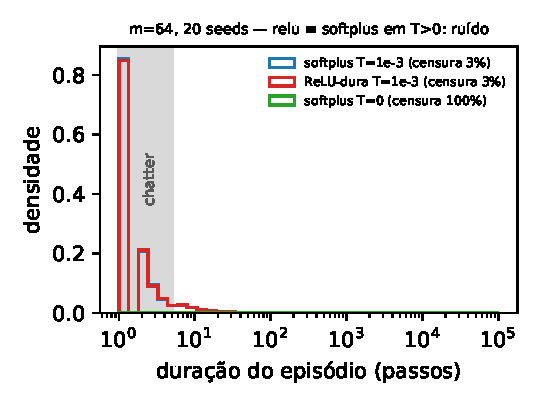
\includegraphics[width=0.56\linewidth]{../../05-experimentos/etapa4-mlp-populacao/fig-diagnostico-duracoes.pdf}
\caption{Why etapa-4a is an instrument negative (post-hoc diagnostic, $m=64$,
$20$ seeds). Episode-duration densities: at $T>0$, hard ReLU $\equiv$ softplus
(median $\sim4$ steps, shaded chatter band) --- a signature of noise, not of the
zero-gradient theorem; the real physics is the $T=0$ arm ($\sim10^3$ steps,
$99.6\%$ censored). Script
\texttt{etapa4-mlp-populacao/figuras\_diagnostico.py}.}
\label{fig:diagnostico}
\end{figure}

A redesign (etapa-4a.2) was itself rejected at the design stage by the same
process (commit \texttt{a413b19}): at $T=10^{-3}$ the ReLU/softplus ratio stayed
$\approx0.95$ after debounce, and an independent replication at the deploy
temperature $T=10^{-5}$ still found ReLU $\approx$ softplus ($7,5$ vs.\ $9,6$
clean episodes) --- gradient starvation at $\beta=300$ masked the effect.
Separately, the pooled null broke $\alpha$ by $30$--$92\times$ in
heterogeneous/autocorrelated worlds, which motivated the per-neuron stratified
null (the stratified version held $\approx\alpha$). The inheritance was explicit: a
hysteresis/dwell ruler, a per-neuron stratified null, and a move to the
deterministic regime $T=0$ with a much longer horizon. These negatives falsify
neither the area law nor the toy calibration; they falsify two rulers, and they
are what forced the working design.

\subsection{The mechanism, observed}\label{sec:mecanismo}

Moving to $T=0$ and a sub-parametrized regime (pressure: a plateau
$\sim0.15$ on the rich target $y=\sin(2\pi x)+0.3\sin(5\pi x)$, $n=16$,
$\eta=10^{-3}$, $H=2\cdot10^5$; $64$ runs, commit \texttt{b48b527}, exploratory)
made the mechanism visible. Hard ReLU gave a \emph{structural zero}: $0$
resurrections out of $25$ deaths in $16$ runs, the frozen ($\mathrm{grad}\equiv0$)
branch exact in a real network at $T=0$. Softplus resurrected by mechanism: at
$\beta=10$ a unit died at step $781$ and returned at $139{,}179$; at $\beta=300$
one died at $3315$ and returned at $152{,}977$ (it had parked shallow enough that
the $e^{\beta z}$ channel did not vanish). Both dynamical resurrections showed the
ordered triple $t_{\mathrm{death}}<t_{\mathrm{area}}<t_{\mathrm{res}}$ (area law
$2/2$). The gate$\to$return gap is the finite-$\beta$ rise time
($\sim|z_{\mathrm{park}}|/\mathrm{drift}$), not the asymptotic $O(1/\beta)$
correction. The bottleneck was quantified as the event rate ($\sim0.1$/run) ---
which set the entire sizing of the confirmatory.

\subsection{Confirmatory: the area law in a real MLP}\label{sec:confirm}

The confirmatory (etapa-4a.3) was pre-registered at commit \texttt{a8f8f8c} after
two more adversarial rounds, with every design number derived programmatically
from a $240$-run rate pilot (commit \texttt{995a87c}); the run is commit
\texttt{5a961cb}. Grade: $\{$sp-$\beta3$ (primary), sp-$\beta10$, sp-$\beta300$,
ReLU$\}\times m\in\{4,6\}\times50$ virgin seeds ($1900$--$1949$) $=400$ runs;
$T=0$, $H=5\cdot10^5$; eligible window $[0,307{,}536]$ ($H-\tau$, $\tau$ the
$q_{0.9}$ return time). The instrument is a single ground-truth clock with
bit-exact parity to the pilot motor; the area of the leader-datum residual is
accumulated on that clock, so temporal ordering is structural and the only
empirical failure mode of the area test is a \emph{return without area}.

\begin{table}[t]
\centering
\small
\begin{tabular}{lccccc}
\toprule
arm & dyn.\ deaths & $\lambda$/run [boot] & returns & $p(\mathrm{ret}\mid\mathrm{death})$ CP & ordered/returns \\
\midrule
sp-$\beta3$   & 35 & 0.350 [0.220,0.500] & 16 & 0.457 [0.288,0.634] & 13/16 \\
sp-$\beta10$  & 27 & 0.270 [0.160,0.390] & 10 & 0.370 [0.194,0.576] & 6/10 \\
sp-$\beta300$ & 19 & 0.190 [0.100,0.290] & 4  & 0.211 [0.061,0.456] & 3/4 \\
ReLU          & 17 & 0.170 [0.090,0.260] & 0  & 0.000 [0.000,0.195] & 0/0 \\
\bottomrule
\end{tabular}
\caption{Confirmatory 4a.3 ($100$ runs/arm, $T=0$). ReLU gives a structural zero
(validity control: any ground-truth return here would invalidate the run).
Clopper--Pearson $95\%$ intervals; bootstrap clustered by seed.}
\label{tab:4a3}
\end{table}

The pre-registered verdicts (Table~\ref{tab:4a3}, Fig.~\ref{fig:escada}):
\begin{itemize}
\item \textbf{C1 (existence with rate, primary sp-$\beta3$): reproduces.}
$N_{\mathrm{elig}}=30$ ($n^\ast=10$), $15$ eligible returns,
$p(\mathrm{ret}\mid\mathrm{eligible})=0.500\ [0.313,0.687]$, well above the kill
threshold $0.076$.
\item \textbf{C2 (the area law, the heart, sp-$\beta3$): sustains.} The
leader-drive area opens before the return in $13/16$ dynamical resurrections
(lower Clopper--Pearson bound $0.544>0.5$, $\ge6$ returns). The $3$
returns-without-area are real and counted against the law (returns driven off the
leader datum --- an object of study, not hidden).
\item \textbf{C4 (channel staircase, estimation, no kill): monotone in $\beta$.}
$p(\mathrm{ret}\mid\mathrm{death})$ falls $0.457>0.370>0.211>0.000$ from
$\beta=3$ to hard ReLU, with intervals --- the activation smoothness controls the
return channel, and $\beta=3$ is the most
alive. This is the direct bridge to the plasticity practice of
\S\ref{sec:noncomm}.
\item \textbf{Validity: clean.} ReLU $0/17$ dynamical returns --- the
non-commutation of Thm.~\ref{thm:main} measured with $N=100$.
\end{itemize}

\begin{figure}[t]
\centering
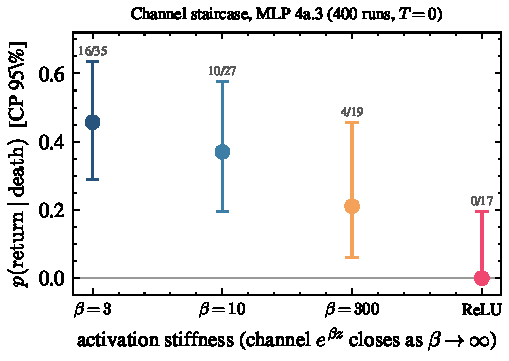
\includegraphics[width=0.56\linewidth]{fig-escada-4a3.pdf}
\caption{The channel staircase (C4, confirmatory 4a.3, $400$ runs, $T=0$).
$p(\mathrm{return}\mid\mathrm{death})$ is monotone in the activation stiffness
and reaches a structural zero at hard ReLU ($\mathrm{grad}\equiv0$); the smooth
channel $e^{\beta z}$ closes as $\beta\to\infty$. Fractions above each point are
returns/deaths; error bars are Clopper--Pearson $95\%$. Script
\texttt{figuras\_paper.py}.}
\label{fig:escada}
\end{figure}

The honest limits of the confirmatory: $T=0$ (deterministic), one small
architecture, a $1$D rich target, $m\in\{4,6\}$. The stochastic regime is a paper
of its own (\S\ref{sec:falsif}). C1's kill is intentionally near-unreachable at
this $N$ (a consequence of the frozen $\tfrac12\times$ pilot-lower-bound rule),
so in practice C2 is the deciding test; this was signalled in the
pre-registration, not discovered after.

\subsection{Confirmatory: two new mechanisms in a one-layer transformer}\label{sec:transformer}

The same question in a one-layer transformer (FFN over an attended token) does
\emph{not} reduce to the MLP, and the scoping (exploratory, commit
\texttt{d4e4c35}) exposed why, with two facts that reshape the confirmatory:

\begin{itemize}
\item \textbf{S1 --- a GELU sign-flip barrier.} $\mathrm{GELU}'(z)$ changes sign
at $z^\ast=-0.7518$ (verified analytically): for $z<z^\ast$ it is negative, so a
deep-dead unit is pushed \emph{away} from the return by its own gradient.
Self-resurrection is possible only in the shallow band $(-0.752,0)$. The
MLP's slope-blind area instrument, ported as is (omitting $g'$), gets the \emph{sign} wrong on $12/12$
GELU episodes; the correct instrument uses the slope-weighted area $A_{\mathrm{drive}}$.
GELU is therefore genuinely outside the monotone-sigmoid class of
Thm.~\ref{thm:main}, not a technicality.
\item \textbf{S2 --- an upstream channel.} The FFN input $h=e+\mathrm{attn}(e)$ is
non-stationary, so a hard-ReLU unit with own-gradient identically zero can still
revive because $h$ moves. With attention frozen the control is exact:
$\Delta\text{margin}=0.000$, $\mathrm{own\_move}=0$; with attention training,
$\mathrm{own\_move}=0$ still but the margin climbs $+0.69$ on average (up to
$+1.32$). The MLP theorem ``dead ReLU $=$ terminal'' holds only when the input is
fixed; the transformer adds a channel the MLP does not have.
\end{itemize}

A rate pilot ($160$ runs, commit \texttt{2dba27d}) then fixed the design: natural
FFN death is $\approx0$ (units in $d=16$ input do not die on their own), so the
confirmatory is necessarily injection-conditional; the non-stationary channel
chatters, forcing a hysteresis instrument ($\delta_h\approx0.0476$, calibrated
from data); the return time is slow ($\tau\approx60$--$66$k), forcing $H=2\cdot10^5$.
The upstream channel was already clean in the pilot ($\Delta=$ train$-$frozen
$=+6/+6/+6/+8$ returns; ReLU $0\to8$ with $\mathrm{own\_move}=0$).

The transformer confirmatory (etapa-5, pre-registered commit \texttt{1b45498};
$800$ runs, $\{$sp-$\beta3$, sp-$\beta10$, GELU, ReLU$\}\times\{$attn-train,
attn-frozen$\}\times$ injection $\{-0.3,-2.0\}\times50$ seeds $2000$--$2049$;
$H=2\cdot10^5$, $T=0$, hysteresis $\delta_h=0.0476$) ran to completion under the
frozen analysis (result commit \texttt{4051e7f}). Its five pre-registered
estimands returned as follows; all counts are of \emph{sustained} returns under
the hysteresis ruler.

\begin{itemize}
\item \textbf{E-A (validity): valid.} Zero sustained returns in relu-frozen
across $100$ injections --- $0/50$ shallow and $0/50$ deep. Own-gradient
$\equiv0$ with a fixed input is terminal, exactly as the theorem requires; any
sustained return here would have invalidated the run.

\item \textbf{E-B (upstream channel): reproduces in all four arms.} With
$\Delta=p_{\mathrm{sust}}(\text{train})-p_{\mathrm{sust}}(\text{frozen})$ and the
bootstrap clustered by seed:
\[
\begin{array}{llr@{\;}c@{\;}l}
\text{sp-}\beta3  & \Delta=0.210\,[0.120,0.300] & (43/100 &\text{vs.}& 22/100),\\
\text{sp-}\beta10 & \Delta=0.200\,[0.110,0.280] & (29/100 &\text{vs.}&  9/100),\\
\text{GELU}       & \Delta=0.220\,[0.120,0.320] & (51/100 &\text{vs.}& 29/100),\\
\text{ReLU}       & \Delta=0.200\,[0.120,0.280] & (20/100 &\text{vs.}&  0/100).
\end{array}
\]
Every lower bound is above zero, and the effect is
\emph{additive and essentially the same}, $\approx+0.20$, across activations
whose own channels differ by orders of magnitude. The ReLU arm is the clean
case: its own channel is exactly zero, so the whole $0\to20/100$ is upstream.
This is a mechanistic answer to why real networks recover dead units even under
hard activations.

\item \textbf{E-C (transfer of the theorem class): transfers.} sp-$\beta3$
frozen with shallow injection --- the FFN's own channel, isolated --- gives
$22/50$ sustained returns, $p_{\mathrm{sust}}=0.440\,[0.300,0.587]$
(Clopper--Pearson), against the pre-registered gate $n^\ast=6$ and kill
threshold $0.0062$. The leader-drive area opens before the return in $21/22$ of
them. This is the direct analogue of the MLP's C2, and it holds.

\item \textbf{E-D (GELU barrier): consistent-with-barrier (confounded with
depth)} --- the pre-registered three-way label, reported verbatim. The counts
are gelu-frozen shallow $29/50$, $0.580\,[0.432,0.718]$, against deep $0/50$,
$0.000\,[0.000,0.071]$; but the depth-matched control sp-$\beta3$-frozen at
$-2.0$ is \emph{also} $0/50$, so the counts alone do not separate the barrier
from injection depth. Indeed the control is uninformative essentially by
construction: at $z=-2$ the softplus own-channel is $\sigma(3z)\approx0.0025$
($0.85\%$ of its shallow value) while $\mathrm{GELU}'(-2)\approx-0.085$ is
adverse --- the depth kills both mechanisms at once. (The rate pilot had
already found a tie at $z=-1.0$, gelu-frozen deep $4/20$ vs.\ shallow $4/20$,
which is why the confirmatory injects at $-2.0$.) The barrier is nonetheless visible in the drive field itself: the
sign inversion $A_{\mathrm{drive}}\neq A_{\mathrm{mlp}}$ occurs in
$46/50=92\%$ of the deep injections against $2/50=4\%$ of the shallow ones. We
therefore report the barrier as \emph{consistent with} the data and visible in
the sign channel --- not as established by the count.

\item \textbf{E-E ($\beta$ staircase, estimation, no kill): monotone.}
$p_{\mathrm{sust}}$ with attention frozen falls from $0.220\,[0.143,0.314]$ at
$\beta=3$ to $0.090\,[0.042,0.164]$ at $\beta=10$; with attention training, from
$0.430\,[0.331,0.533]$ to $0.290\,[0.204,0.389]$. The MLP staircase of
\S\ref{sec:confirm} reappears in the transformer, in both the own and the
upstream regimes: stiffening the activation closes the return channel.
\end{itemize}

Across the grid the drive area opens before the return in the
large majority of sustained returns --- $21/22$ (sp-$\beta3$ frozen), $34/39$
(sp-$\beta3$ train), $26/27$ (sp-$\beta10$ train), $24/29$ (GELU frozen) ---
as in the MLP.

The scoping verdict survives the confirmatory and is itself a result: the MLP
mechanism does not transfer directly to the GELU FFN --- the sign-flip barrier
obstructs self-resurrection --- while the theorem's own class (softplus-$\beta$)
does transfer, and the upstream channel is a genuinely new route that the MLP
does not have. The confirmatory is injection-conditional by design (natural FFN
death is $\approx0$ at $d=16$), so it measures the fate of units placed dead,
not the rate at which they die.

\section{Limitations}\label{sec:limits}

We state them explicitly. \textbf{(i)} The theorem is proved for one two-neuron
instance; every constant is verified there and breadth is future work.
\textbf{(ii)} The regime is $T=0$ deterministic gradient flow throughout the
theorem and both confirmatories; the stochastic (SGLD) gate is open and, where
probed, \emph{falsifies} the deterministic schedule (\S\ref{sec:falsif}) --- late
captures recur past the deterministic window at a rate the reduced stochastic
model under-predicts, leaving the reactivating unit's back-reaction as the
leading candidate driver. \textbf{(iii)} Scale: the confirmatories are small
networks ($m\le6$ MLP units, $m_{\mathrm{ffn}}=4$ FFN units) with rich $1$D
targets, chosen so that a single unit can be tracked with a ground-truth clock.
\textbf{(iv)} The transformer confirmatory is \emph{injection-conditional}:
natural FFN death is $\approx0$ at $d=16$, so it measures the fate of units
placed dead, not the rate at which they die; the design declares this and does
not claim a death rate. \textbf{(v)} GELU is outside the monotone class, and our
transformer verdict on its barrier is \emph{consistent with}, not established:
the deep-vs-shallow count is confounded with injection depth (the depth-matched
softplus control is also $0/50$), and the sign signature shows the barrier acting in the drive field without separating it from depth
(\S\ref{sec:transformer}). \textbf{(vi)} The cone apex
(corank $\ge2$), where weight decay produces genuine sliding toward the most
singular stratum, is untouched.

\section{Reproducibility}\label{sec:repro}

All runs are deterministic on CPU with per-run manifests (SHA256 + git + config);
raw episode files and aggregate JSON are committed alongside the code.
Pre-registration commits precede every confirmatory run in the repository history.

{\sloppy
\begin{itemize}
\item \textbf{Theorem constants and figures.} \texttt{06-notas/t2-prova/}: lemma
verifications \texttt{passo0--6.py}, \texttt{prova\_L1--L6.py}; figures via
\texttt{figuras\_draft.py}.
\item \textbf{MLP mechanism (pilot).}
\texttt{etapa4-mlp-populacao/pilotos-4a2/pressao/}; commit \texttt{b48b527}.
\item \textbf{MLP confirmatory (4a.3).} \texttt{.../pressao/taxa/}: pre-registration
\texttt{a8f8f8c}, run \texttt{5a961cb}. \\
\texttt{python run\_4a3.py --workers 4} then \texttt{python analise\_4a3.py}
(reads \texttt{results-4a3/} + \texttt{config\_4a3.json}). Rate pilot
\texttt{995a87c}. Staircase figure: \texttt{06-notas/paper/figuras\_paper.py}.
\item \textbf{Transformer confirmatory (etapa-5).}
\texttt{05-experimentos/etapa5-transformer/}: scoping \texttt{d4e4c35}, rate
pilot \texttt{2dba27d}, confirmatory pre-registration \texttt{1b45498} (which
freezes \texttt{config\_e5.json}: $\delta_h=0.0476$, $800$ runs, seeds
$2000$--$2049$, $H=2\cdot10^5$), result commit \texttt{4051e7f}. \\
\texttt{python run\_e5.py --workers 4} then \texttt{python analise\_e5.py}
(reads \texttt{results-e5/}, $800$ episode files $+$ manifest, and writes
\texttt{resultado-e5.md}).
\item \textbf{Negatives.} \texttt{05-experimentos/NEGATIVOS.md} and the etapa-4a
note record the invalidated instrument (commit \texttt{6411ac8}) and the rejected
redesign (\texttt{a413b19}); the falsified schedule is
\texttt{p5-relu-morte-v2/} (commit \texttt{190d94a}).
\end{itemize}
\par}

\appendix
\section{The six lemmas}\label{app:lemmas}

\begin{lemma}[normal form]\label{lem:gauge}
In the gauge $w=e^{\beta z}$, fast time $\tau=\beta t$:
$dw/d\tau=cR(t)\,w^2/(1+w)\,(1+E_\beta)$, $|E_\beta|\le\log(1+w)/(\beta|R|)$ ---
the quadratic normal form of De Maesschalck--Schecter~\cite{DMS16} with
$\varepsilon=\beta^{-1}$. With $u=1/w$ and $\Phi(u)=\log u+u$ one has the exact
quadrature $d\Phi/dt=-c\beta R(t)(1+E_\beta)$.
\end{lemma}

\begin{lemma}[$B$-subsystem and feedback]\label{lem:gronwall}
Under (H4) the $B$-field is affine with Lipschitz constant
$L_B=\lambda_{\max}(G_B)$ and $R^{\mathrm{hyb}}$ is affine in $\theta_B$. Integral
Gr\"onwall consuming the bound of Lem.~\ref{lem:gauge} gives, conditionally on the
layer being maintained (supplied by Lem.~\ref{lem:bootstrap}), the refined rate
$\sup\|\theta_B^\beta-\theta_B^{\mathrm{hyb}}\|=O(\log\beta/\beta^{2})$ --- one
full order better than the naive $O(\beta^{-1})$: in the bulk $u=O(\beta|A|)$, so
the coupling is $O(\beta^{-2})$ there and $O(\beta^{-1})$ only in the
$O(\beta^{-1})$-wide corner windows. Verified: metric
$\sup\cdot\beta^2/\log\beta$ stable in $[4.2,5.7]$.
\end{lemma}

\begin{lemma}[entry corner]\label{lem:corner-in}
$\dot z^0(\thit^-)=cR^{\mathrm{hyb}}(\thit)<0$ by (H1). The exact identity
$(1-\sigma)/\sigma=e^{-s}$ collapses the crossing-time difference to an elementary
integral: $t_{\mathrm{cross}}^\beta=\thit+\tfrac{1}{\beta v}(1+O(\delta_z)+o(1))$
with $v=c|R^{\mathrm{hyb}}(\thit)|$, and the exponentially weighted approach
integral is $\tfrac{3/2}{\beta v}(1+o(1))$. Verified: $K_{\mathrm{teo}}=7.04$ vs
$K_{\mathrm{emp}}=7.13$ ($1.2\%$); weight constant to $<1\%$.
\end{lemma}

\begin{lemma}[sticking and release, prescribed $R$]\label{lem:release}
For prescribed $R$ satisfying (H1)--(H2), with $A(t)=\int_{\thit}^t R$: the exact
additive identity $d\Phi/dt=-c\beta R+c\log(1+w)$ holds (no division by $R$; the
interior zero of $R$ forced by (H1)--(H2) is harmless --- the layer is held by
the \emph{area}, not the sign of $R$), and on compact subintervals of
$(\thit,\texit)$, $\Phi(u(t))=-c\beta A(t)(1+o(1))$, hence
$u(t)=c\beta|A(t)|(1+o(1))$ (depth $z\sim-\beta^{-1}\log\beta$), and $u$ returns
to $O(1)$ at $\texit+O(\beta^{-1})$ --- no $\log\beta$ factor. Sub/super solutions
from monotonicity in $R$ give explicit constants; a perturbation $\delta$ of $R$
shifts $\texit$ by $\le c\,\delta\,(\texit-\thit)/|A'(\texit)|+O(\delta^2)$.
\end{lemma}

\begin{lemma}[coupled bootstrap]\label{lem:bootstrap}
Continuation with strict margins: the property ``$\theta_B$ is
$2M_2\log\beta/\beta^2$-close to the hybrid and the margin stays strictly in the
layer after an $O(\beta^{-1})$ entry collar'' is nonempty
(Lem.~\ref{lem:corner-in}), open (strict inequalities $+$ continuity) and closed
(the assumption returns the better constant $M_2$ via Lem.~\ref{lem:gronwall},
and Lem.~\ref{lem:release} with $\delta=O(\log\beta/\beta^2)$ keeps the layer up
to $\texit-C_\varepsilon\log\beta/\beta$), with $M_2=e^{L_BT}C_fC_4/c$ independent
of the hypothesis for $\beta\ge\beta_0$ (a finite threshold traceable through the constant chain, not exhibited; the strict layer check is vacuous for $\beta\le3\cdot10^3$ under the conservative $C_\varepsilon$ and confirmed at $\beta=10^4$); with the empirical $C_4=10.6$,
$M_2=440.8$; the leading term of the theoretical $C_4$ is
$2/(cR^{\mathrm{hyb}}(\texit))=29.6$. The entry corner cuts initial area
$\approx R^{\mathrm{hyb}}(\thit)K/\beta$, advancing the exit by
$1/(cR^{\mathrm{hyb}}(\texit)\beta)$ --- the arrival speed cancels. Hence the
two-term closed-loop law
$\beta(t^\beta_{\mathrm{release}}-\texit)=(-1+\mathrm{corr}(\beta))/(cR^{\mathrm{hyb}}(\texit))+o(1)$.
Verified: the two-term law reproduces the entire coupled sweep at
$1.9\%/0.7\%/0.2\%/0.1\%$ ($\beta=3\cdot10^2\ldots10^4$).
\end{lemma}

\begin{lemma}[exit corner; scalar reduction]\label{lem:corner-out}
Post-release the field is transversal outward ($cR^{\mathrm{hyb}}(\texit)>0$,
(H2)); the mirrored corner identities of Lem.~\ref{lem:corner-in} apply with
$v'=cR^{\mathrm{hyb}}(\texit)$. Forward uniqueness of the restarted ReLU flow
holds on the \emph{activating branch}, selected by the limit itself (release at
$\texit+O(\beta^{-1})$ is incompatible with the frozen Filippov branch);
classical Gr\"onwall glues on $[\trel,T]$ at rate $O(\log\beta/\beta)$. Under (H3)
the other data contribute $O(e^{-\beta\delta_1})$, the face-$j$ field is rank one
along $(x_j,1)$, and the episode reduces to the scalar problem. Verified: gluing
sup $=1.6\cdot10^{-3}/5.5\cdot10^{-4}$ at $\beta=10^3/3\cdot10^3$.
\end{lemma}

\begin{thebibliography}{99}
\bibitem{DMS16} P.~De Maesschalck, S.~Schecter, \emph{The entry--exit function
and geometric singular perturbation theory}, J.~Diff.~Eq.\ 260 (2016) 6697--6715.
\bibitem{Kri17} K.~U.~Kristiansen, \emph{Blowup for flat slow manifolds},
Nonlinearity (2017); arXiv:1603.01821.
\bibitem{GH} N.~Guglielmi, E.~Hairer, \emph{On the limit solution of regularized
piecewise-smooth dynamical systems}, preprint, Univ.\ Geneva, 2019; foundational
results in SIAM J.~Appl.~Dyn.~Syst.\ 14 (2015) 1454--1477.
\bibitem{Jef16} M.~R.~Jeffrey, \emph{Exit from sliding in piecewise-smooth flows:
deterministic vs.\ determinacy-breaking}, Chaos 26 (2016) 033108.
\bibitem{SDR23} M.~Sensi, M.~Desroches, S.~Rodrigues, \emph{Slow-fast dynamics in
a neurotransmitter release model: delayed response to a time-dependent input
signal}, Physica D (2023); arXiv:2302.12852.
\bibitem{ST98} J.~Sotomayor, M.~A.~Teixeira, \emph{Regularization of
discontinuous vector fields}, in: Int.\ Conf.\ on Differential Equations
(Lisboa 1995), World Scientific, 1998, pp.~207--223.
\bibitem{LST07} J.~Llibre, P.~R.~da Silva, M.~A.~Teixeira, \emph{Regularization of
discontinuous vector fields on $\mathbb{R}^3$ via singular perturbation},
J.~Dynam.~Differential Equations 19 (2007) 309--331.
\bibitem{EJRW23} S.~Eberle, A.~Jentzen, A.~Riekert, G.~S.~Weiss, \emph{Existence,
uniqueness, and convergence rates for gradient flows in the training of
artificial neural networks with ReLU activation}, Electron.~Res.~Arch.\ 31 (2023)
2519--2554; arXiv:2108.08106.
\bibitem{Sokar23} G.~Sokar, R.~Agarwal, P.~S.~Castro, U.~Evci, \emph{The dormant
neuron phenomenon in deep reinforcement learning}, ICML 2023; arXiv:2302.12902.
\bibitem{Lyle23} C.~Lyle, Z.~Zheng, E.~Nikishin, B.~Avila Pires, R.~Pascanu,
W.~Dabney, \emph{Understanding plasticity in neural networks}, ICML 2023;
arXiv:2303.01486.
\bibitem{Dohare24} S.~Dohare, J.~F.~Hernandez-Garcia, Q.~Lan, P.~Rahman,
A.~R.~Mahmood, R.~S.~Sutton, \emph{Loss of plasticity in deep continual
learning}, Nature 632 (2024) 768--774.
\end{thebibliography}

\end{document}
